% !TEX root = main.tex
\section{Problem Overview}

An end-to-end robotic system consist of cascade of modules which are designed to enable specific robotic abilities such as grasping, path planning, language understanding etc. In this
work we address the problem of learning such end-to-end systems in an interactive manner with a human-in-the-loop. We want the interactive learning procedure to be easy for any non-expert user to use. Such non-expert users are typically agnostic to the individual modules involved in the overall robotic system and therefore cannot manually tune each module. In fact they can at best judge the final behaviour produced by the robot. We propose an interactive procedure, where by simply observing user feedback on the final output produced by the robot, the entire robotic system can be learned.

In our formulation we consider cascade of modules that accomplish a robotic task, where the output of one module forms the input to the module following it. The input into the cascade is a robotic task which is then forward propagated through multiple modules. The last module in the cascade generates the final robot behaviour which is visible to the user e.g. a trajectory accomplishing the task. In our learning setting, we elicit a \textit{coactive feedback} from the user on the final robot behaviour. Through this feedback the user slightly improves upon the output produced by the robot, but never reveals the optimal behaviour. Our feedback mechanism has certain desirable characteristics: (i) it is \textit{weak}, in the sense the non-expert user never reveals the optimal behaviour to the robot; and (ii) it is \textit{global}, in the sense the user does not provide feedback at the module level and only improves upon the final robot behaviour. The \textit{global} nature of feedback makes learning challenging since the user feedback needs to be distributed to each module. We now formally define the learning setting.

\section{System Overview}
System consists of an interactive web based interface where user can see the robotic tasks
executed for a particular NLP instruction. User can give their like and dislike
over this output. User can also provide a more detailed feedback whereby user stops the robot, drags it and thus updates the robot trajectory. In the present work, we work with the detailed feedback and aim to utilise the weak like dislike feedback in the future work.

\begin{figure}[h]
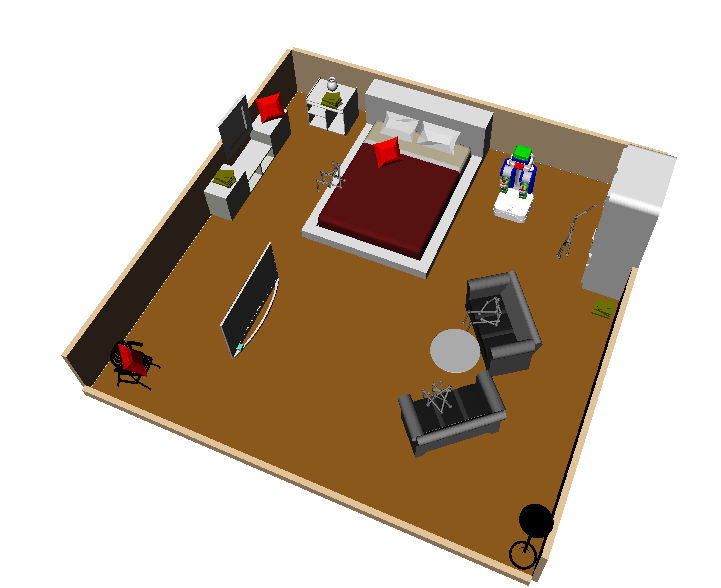
\includegraphics[width=8cm]{env}
\centering
\caption{Robotic simulator to capture user feedback}
	\label{fig:env}
\end{figure}
